\section{Variable Neighborhood Descent (VND)}
\label{sec:vnd}

O \emph{Variable Neighborhood Descent} (VND) aplica descida local em uma sequência finita de vizinhanças e reinicia da primeira ao encontrar melhoria \cite{hansen2001variable}. No VRPTW, essa estratégia permite combinar movimentos baratos (intra-rota) com movimentos estruturais (inter-rotas), mantendo controle sobre factibilidade temporal e custo.

\subsection{Estratégia implementada}

A implementação adota o padrão clássico com política \emph{first improvement}:
\begin{itemize}
  \item para uma vizinhança $\mathcal{N}_k$, a busca encerra assim que encontra o primeiro movimento factível com melhora;
  \item quando há melhora, o algoritmo volta para $\mathcal{N}_1$;
  \item quando não há melhora, avança para $\mathcal{N}_{k+1}$.
\end{itemize}

\begin{algorithm}[htbp]
\caption{VND com \emph{first improvement}}
\label{alg:vnd}
\begin{algorithmic}[1]
\Require solução inicial $S$, vizinhanças ordenadas $\mathcal{N}_1,\ldots,\mathcal{N}_K$
\Ensure ótimo local $S^*$ para o conjunto de vizinhanças
\State $k \leftarrow 1$
\While{$k \le K$}
  \If{\textsc{FirstImprove}$(S,\mathcal{N}_k)$}
    \State $k \leftarrow 1$
  \Else
    \State $k \leftarrow k + 1$
  \EndIf
\EndWhile
\State \Return $S$
\end{algorithmic}
\end{algorithm}

\paragraph{Texto complementar ao pseudocódigo.}
No código, a rotina \textsc{FirstImprove} é especializada por operador (não é uma função genérica). Em todos os casos, a lógica é a mesma: enumerar movimentos candidatos, testar factibilidade e aceitar o primeiro que satisfaça a regra de melhora. O teste de factibilidade inclui capacidade e janelas de tempo via recálculo de cronograma da(s) rota(s) afetada(s), de modo que nenhum movimento inviável é aplicado. A comparação de qualidade é lexicográfica: primeiro custo total, depois número de rotas. Assim, as linhas 2--7 do Algoritmo~\ref{alg:vnd} representam exatamente o comportamento implementado em \texttt{src/heuristics/local\_search.cpp}: \emph{melhorou} $\Rightarrow$ reinicia; \emph{não melhorou} $\Rightarrow$ troca de vizinhança.

\paragraph{Conformidade DIMACS e desempate secundário.}
Em estrita conformidade com o 12º Desafio DIMACS, a função objetivo primária do framework é a minimização da distância total (\texttt{--objective cost}). Como critério secundário de aceitação (desempate lexicográfico), um movimento com variação de custo dentro da tolerância numérica $\varepsilon$ só é aceito se reduzir o número de rotas. Essa regra preserva o foco primário em distância e, ao mesmo tempo, aumenta a robustez estrutural das soluções ao eliminar rotas residuais sem alterar o orçamento de busca.

\subsection{Conjunto de vizinhanças ativas}
\label{subsec:vnd_neighborhoods}

A versão final usa quatro vizinhanças:
\begin{enumerate}
  \item \texttt{relocate\_intra}: desloca um cliente para outra posição da mesma rota;
  \item \texttt{swap\_intra}: troca duas posições na mesma rota;
  \item \texttt{relocate\_inter}: move um cliente de uma rota para outra;
  \item \texttt{or\_opt}: move bloco consecutivo de tamanho 2 ou 3 (intra e inter-rotas).
\end{enumerate}

A ordem no código é fixa:
\[
\mathcal{N}_1=\texttt{relocate\_intra},\;
\mathcal{N}_2=\texttt{swap\_intra},\;
\mathcal{N}_3=\texttt{relocate\_inter},\;
\mathcal{N}_4=\texttt{or\_opt}.
\]

Um movimento $m$ que transforma $S$ em $S'$ só é aceito se:
\[
\text{factível}(S') \;\land\;
\Big(f(S') < f(S)-\varepsilon \;\;\lor\;\; (|R(S')|<|R(S)| \land |f(S')-f(S)|\le\varepsilon)\Big),
\]
em que $f(\cdot)$ é o custo total e $|R(\cdot)|$ é o número de rotas.

\subsection{Representação visual das vizinhanças}
\label{subsec:vnd_figuras}

As figuras abaixo mostram exemplos didáticos de cada operador ativo (antes/depois). O mesmo desenho foi gerado em duas versões: PNG (usada no PDF) e SVG vetorial (em \texttt{artigo/figs/svg/}), para uso em apresentações sem perda de qualidade.

\begin{figure}[htbp]
\centering
\IfFileExists{figs/png/vnd_relocate_intra.png}{
  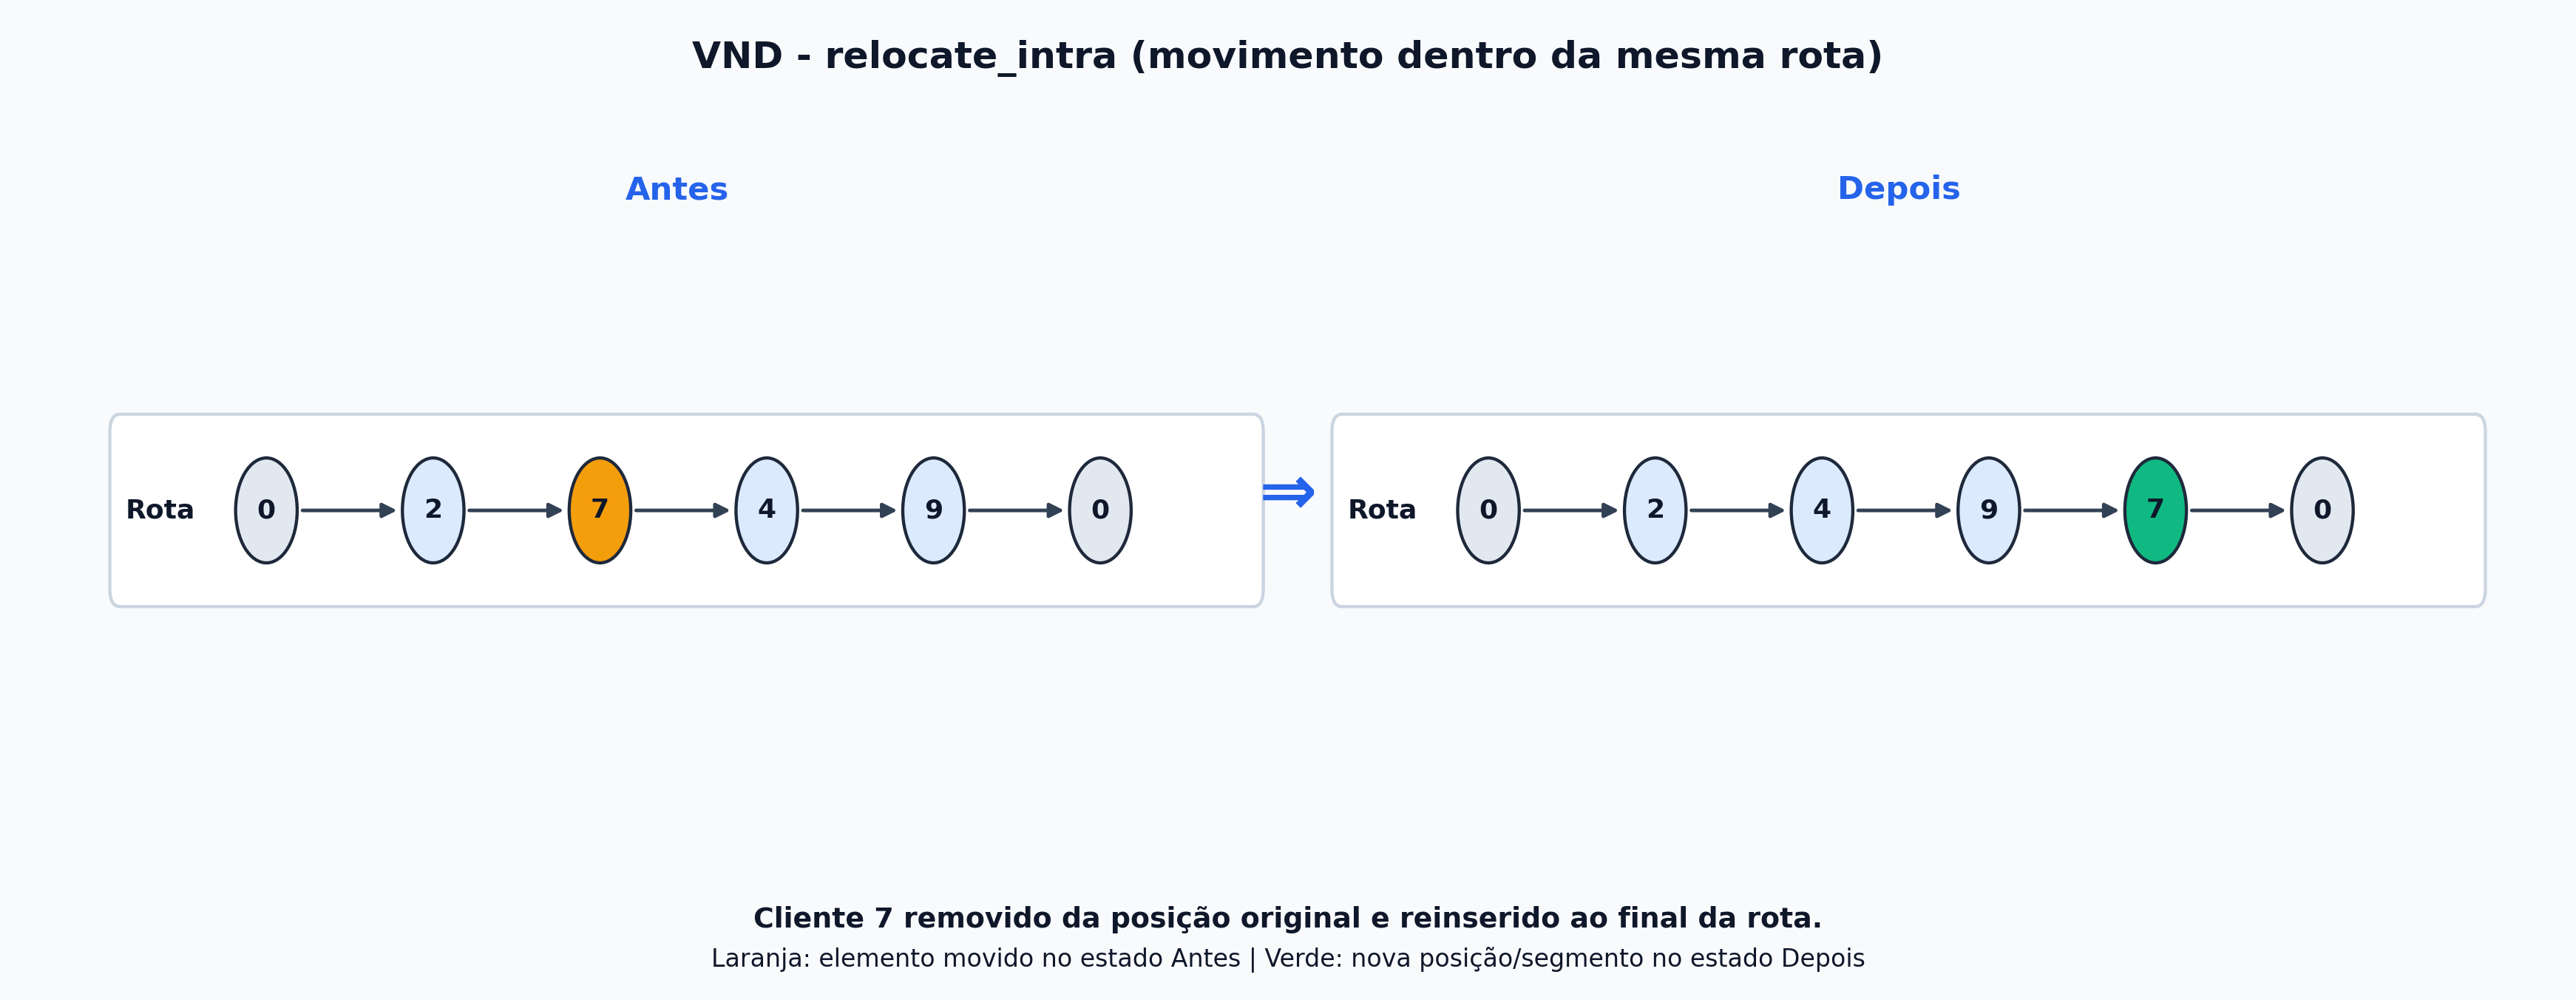
\includegraphics[width=0.96\linewidth]{figs/png/vnd_relocate_intra.png}
}{
  \fbox{\parbox{0.92\linewidth}{Figura ausente: execute \texttt{python3 artigo/figs/generate\_vnd\_figures.py}.}}
}
\caption{\texttt{relocate\_intra}: um cliente é removido de sua posição original e reinserido em outra posição da mesma rota.}
\label{fig:vnd_relocate_intra}
\end{figure}

\begin{figure}[htbp]
\centering
\IfFileExists{figs/png/vnd_swap_intra.png}{
  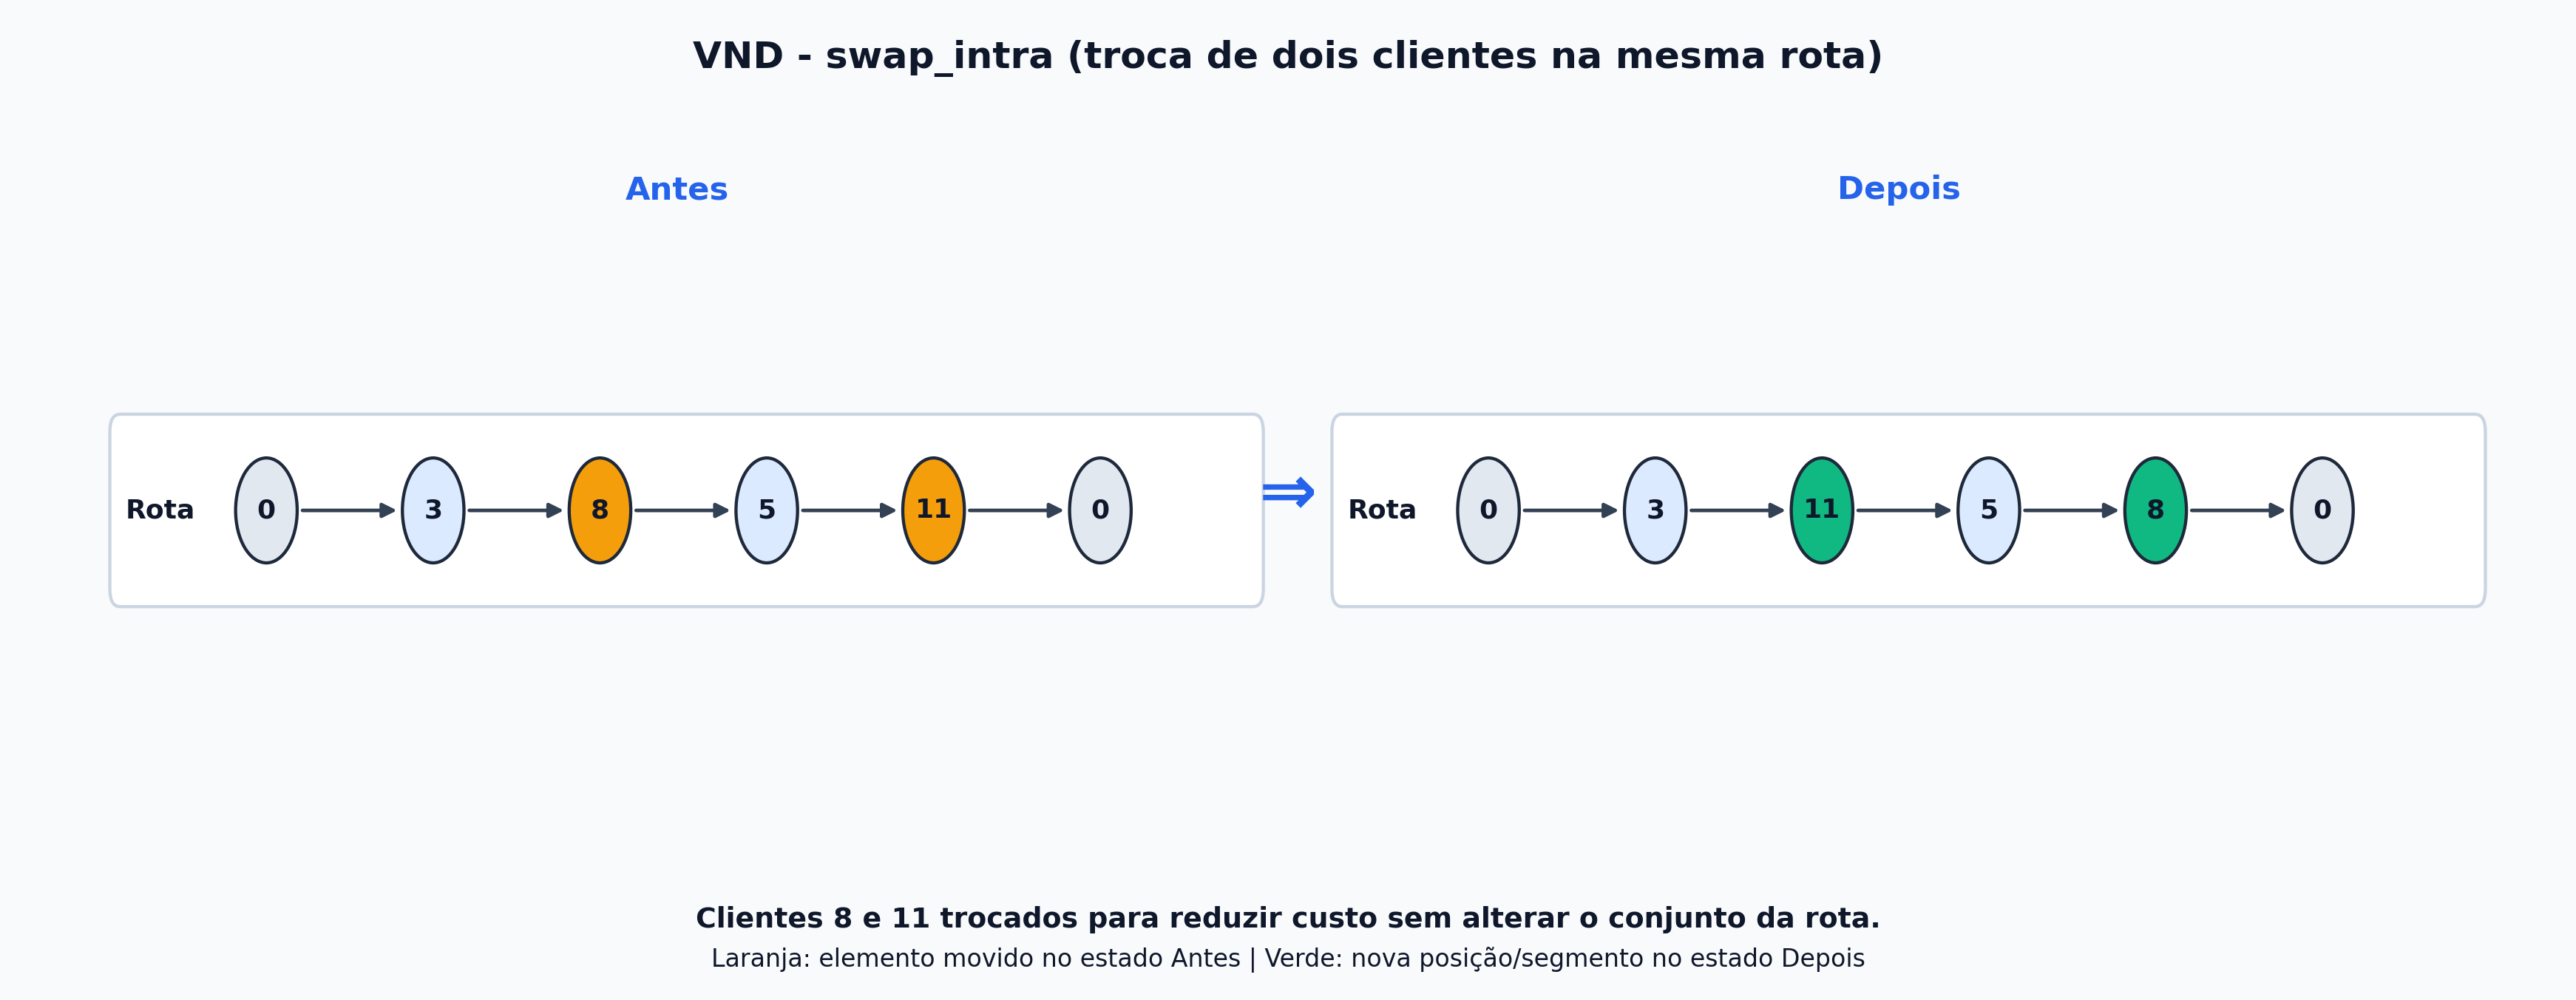
\includegraphics[width=0.96\linewidth]{figs/png/vnd_swap_intra.png}
}{
  \fbox{\parbox{0.92\linewidth}{Figura ausente: execute \texttt{python3 artigo/figs/generate\_vnd\_figures.py}.}}
}
\caption{\texttt{swap\_intra}: dois clientes trocam de posição dentro da mesma rota.}
\label{fig:vnd_swap_intra}
\end{figure}

\begin{figure}[htbp]
\centering
\IfFileExists{figs/png/vnd_relocate_inter.png}{
  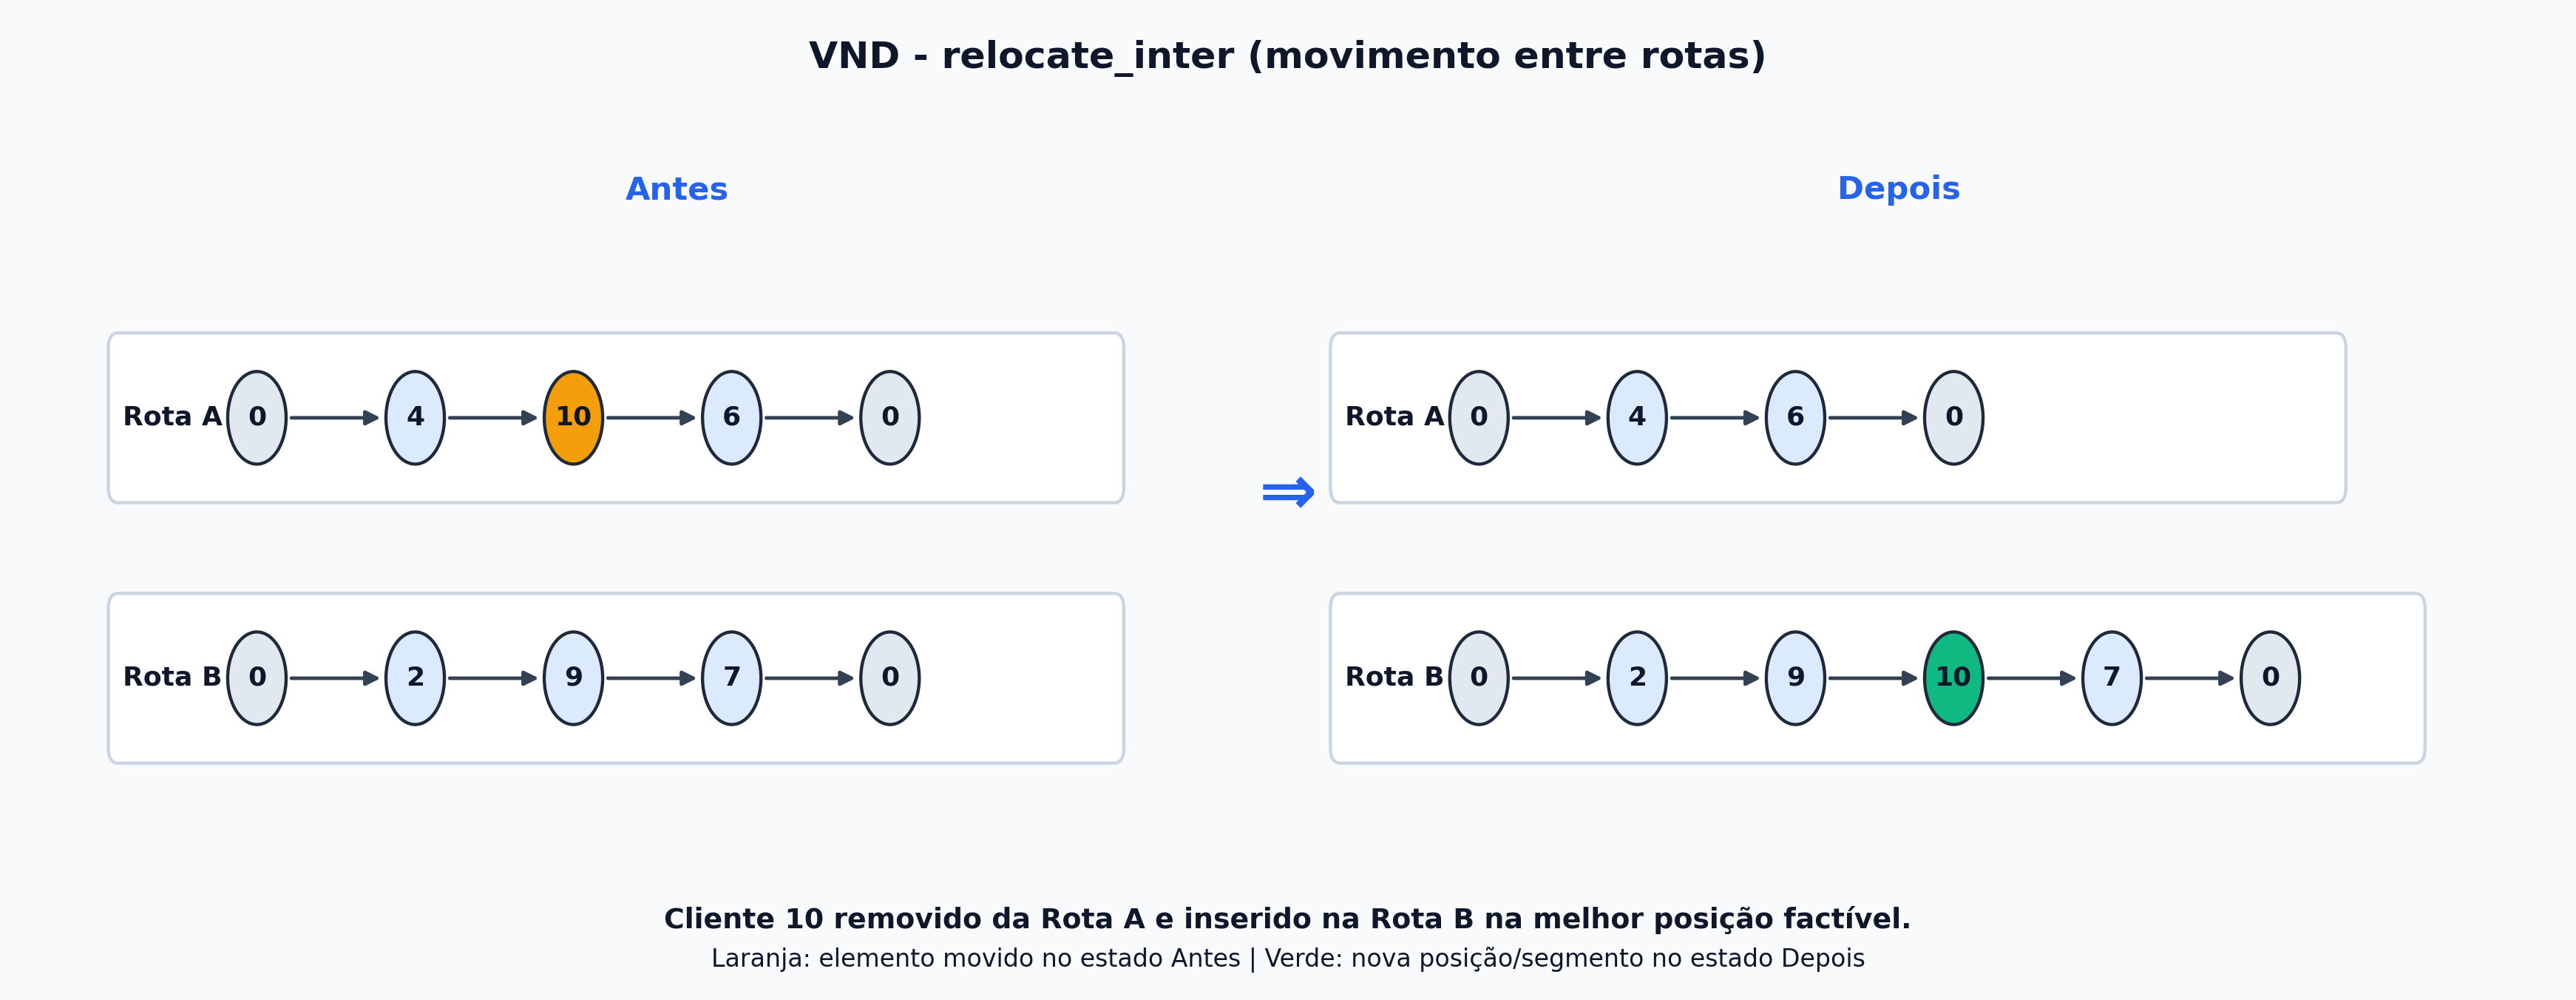
\includegraphics[width=0.96\linewidth]{figs/png/vnd_relocate_inter.png}
}{
  \fbox{\parbox{0.92\linewidth}{Figura ausente: execute \texttt{python3 artigo/figs/generate\_vnd\_figures.py}.}}
}
\caption{\texttt{relocate\_inter}: um cliente sai da rota de origem e é inserido na melhor posição factível de outra rota.}
\label{fig:vnd_relocate_inter}
\end{figure}

\begin{figure}[htbp]
\centering
\IfFileExists{figs/png/vnd_or_opt.png}{
  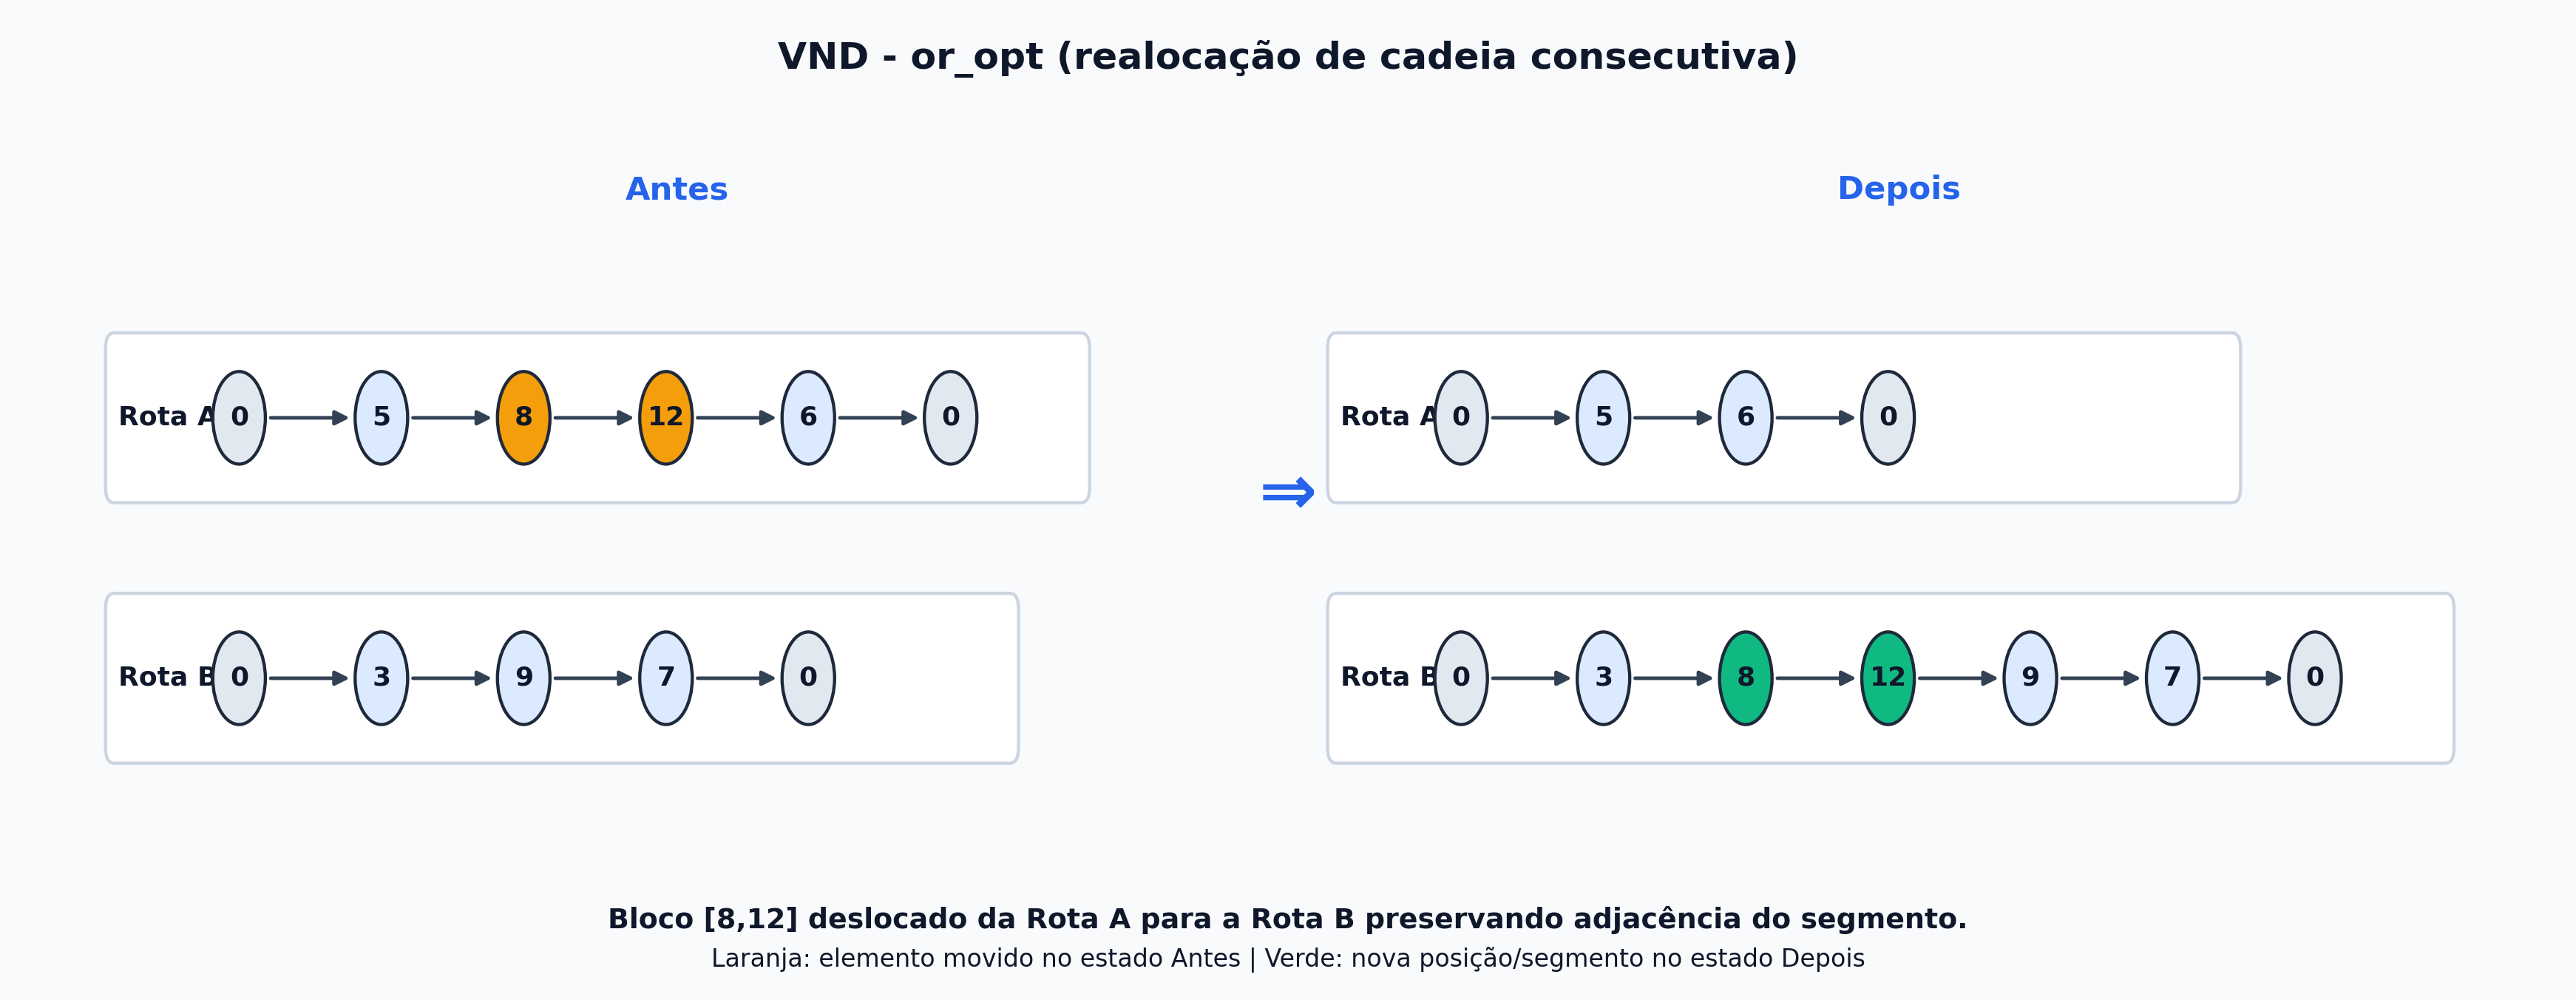
\includegraphics[width=0.96\linewidth]{figs/png/vnd_or_opt.png}
}{
  \fbox{\parbox{0.92\linewidth}{Figura ausente: execute \texttt{python3 artigo/figs/generate\_vnd\_figures.py}.}}
}
\caption{\texttt{or\_opt}: bloco consecutivo (tamanho 2 ou 3) é deslocado de forma íntegra para nova posição factível.}
\label{fig:vnd_or_opt}
\end{figure}

\subsection{Seleção de 4 vizinhanças a partir de 8 candidatas}

A redução de 8 para 4 vizinhanças foi baseada em campanha empírica com 56 instâncias e 10 sementes (560 execuções), usando ganho acumulado de custo por operador. A Tabela~\ref{tab:vnd_impact_global} resume o ranking global.

\IfFileExists{tables/vnd_neighborhood_results.tex}{
% Auto-generated by scripts/build_vnd_neighborhood_table.py
\begin{table}[htbp]
\centering
\caption{Resultados por vizinhança implementada no VND (560 execuções).}
\label{tab:vnd_impact_global}
\begin{tabular}{lrrrrr}
\hline
Vizinhança & Tentativas & Aplicações & Taxa (\%) & $\Delta$ custo total & Share (\%) \\
\hline
relocate\_intra & 35590 & 19050 & 53.53 & 63842.0 & 47.14 \\
relocate\_inter & 9480 & 7700 & 81.22 & 31012.0 & 22.90 \\
or\_opt & 14810 & 5330 & 35.99 & 29997.0 & 22.15 \\
swap\_intra & 16540 & 1110 & 6.71 & 3207.0 & 2.37 \\
two\_opt\_star\_inter & 1170 & 590 & 50.43 & 2913.0 & 2.15 \\
swap\_inter & 1780 & 610 & 34.27 & 2270.0 & 1.68 \\
two\_opt\_intra & 15430 & 620 & 4.02 & 2016.0 & 1.49 \\
cross\_exchange & 580 & 20 & 3.45 & 181.0 & 0.13 \\
\hline
\end{tabular}
\end{table}

}{
\begin{table}[htbp]
\centering
\caption{Impacto global das vizinhanças do VND (560 execuções).}
\label{tab:vnd_impact_global}
\begin{tabular}{lrrrr}
\hline
Vizinhança & Share (\%) & $\Delta$ custo total & Aplicações & Taxa de aplicação (\%) \\
\hline
relocate\_intra & 47.14 & 63842.0 & 19050 & 53.53 \\
relocate\_inter & 22.90 & 31012.0 & 7700 & 81.22 \\
or\_opt & 22.15 & 29997.0 & 5330 & 35.99 \\
swap\_intra & 2.37 & 3207.0 & 1110 & 6.71 \\
two\_opt\_star\_inter & 2.15 & 2913.0 & 590 & 50.43 \\
swap\_inter & 1.68 & 2270.0 & 610 & 34.27 \\
two\_opt\_intra & 1.49 & 2016.0 & 620 & 4.02 \\
cross\_exchange & 0.13 & 181.0 & 20 & 3.45 \\
\hline
\end{tabular}
\end{table}
}

As quatro vizinhanças mantidas cobrem 94.55\% do ganho total observado. Com isso, o VND final reduz custo computacional e mantém praticamente todo o potencial de melhoria do conjunto completo.

\subsection{Resultados por tipo de instância}

Para detalhar o comportamento por família do benchmark Solomon, a Tabela~\ref{tab:vnd_impact_c}, a Tabela~\ref{tab:vnd_impact_r} e a Tabela~\ref{tab:vnd_impact_rc} apresentam os resultados das vizinhanças implementadas separadamente para instâncias C, R e RC.

\IfFileExists{tables/vnd_neighborhood_results_by_family.tex}{
% Auto-generated by scripts/build_vnd_neighborhood_tables_by_family.py
\begin{table}[htbp]
\centering
\caption{Resultados por vizinhança implementada no VND para a família C.}
\label{tab:vnd_impact_c}
\begin{tabular}{lrrrrr}
\hline
Vizinhança & Tentativas & Aplicações & Taxa (\%) & $\Delta$ custo total & Share (\%) \\
\hline
relocate\_inter & 1450 & 1080 & 74.48 & 8505.0 & 35.34 \\
relocate\_intra & 5390 & 2840 & 52.69 & 8188.0 & 34.03 \\
or\_opt & 2210 & 760 & 34.39 & 4743.0 & 19.71 \\
swap\_intra & 2550 & 290 & 11.37 & 1352.0 & 5.62 \\
two\_opt\_star\_inter & 260 & 90 & 34.62 & 579.0 & 2.41 \\
swap\_inter & 370 & 110 & 29.73 & 432.0 & 1.80 \\
two\_opt\_intra & 2260 & 50 & 2.21 & 264.0 & 1.10 \\
cross\_exchange & 170 & 0 & 0.00 & 0.0 & 0.00 \\
\hline
\end{tabular}
\end{table}

\begin{table}[htbp]
\centering
\caption{Resultados por vizinhança implementada no VND para a família R.}
\label{tab:vnd_impact_r}
\begin{tabular}{lrrrrr}
\hline
Vizinhança & Tentativas & Aplicações & Taxa (\%) & $\Delta$ custo total & Share (\%) \\
\hline
relocate\_intra & 17960 & 9150 & 50.95 & 28919.0 & 48.14 \\
relocate\_inter & 5300 & 4410 & 83.21 & 13271.0 & 22.09 \\
or\_opt & 7960 & 2660 & 33.42 & 13005.0 & 21.65 \\
two\_opt\_star\_inter & 590 & 340 & 57.63 & 1627.0 & 2.71 \\
two\_opt\_intra & 8330 & 370 & 4.44 & 1099.0 & 1.83 \\
swap\_intra & 8810 & 480 & 5.45 & 992.0 & 1.65 \\
swap\_inter & 890 & 300 & 33.71 & 983.0 & 1.64 \\
cross\_exchange & 250 & 20 & 8.00 & 181.0 & 0.30 \\
\hline
\end{tabular}
\end{table}

\begin{table}[htbp]
\centering
\caption{Resultados por vizinhança implementada no VND para a família RC.}
\label{tab:vnd_impact_rc}
\begin{tabular}{lrrrrr}
\hline
Vizinhança & Tentativas & Aplicações & Taxa (\%) & $\Delta$ custo total & Share (\%) \\
\hline
relocate\_intra & 12240 & 7060 & 57.68 & 26735.0 & 52.12 \\
or\_opt & 4640 & 1910 & 41.16 & 12249.0 & 23.88 \\
relocate\_inter & 2730 & 2210 & 80.95 & 9236.0 & 18.00 \\
swap\_intra & 5180 & 340 & 6.56 & 863.0 & 1.68 \\
swap\_inter & 520 & 200 & 38.46 & 855.0 & 1.67 \\
two\_opt\_star\_inter & 320 & 160 & 50.00 & 707.0 & 1.38 \\
two\_opt\_intra & 4840 & 200 & 4.13 & 653.0 & 1.27 \\
cross\_exchange & 160 & 0 & 0.00 & 0.0 & 0.00 \\
\hline
\end{tabular}
\end{table}


}{
\begin{table}[htbp]
\centering
\caption{Resultados por tipo de instância (pendente de geração).}
\begin{tabular}{lc}
\hline
Status & Observação \\
\hline
Pendente & Execute \texttt{python3 scripts/build\_vnd\_neighborhood\_tables\_by\_family.py}. \\
\hline
\end{tabular}
\end{table}
}
